\epigraph{The Babel fish is small, yellow, leech-like, and probably the oddest
thing in the universe. It feeds on brainwave energy  ...
%absorbing all unconscious
%frequencies and then excreting telepathically a matrix formed from the conscious
%frequencies and nerve signals picked up from the speech centres of the brain,
%the practical upshot of which is that 
if you stick a Babel fish in your ear, you can
instantly understand anything in any form of language.}{{\it The Hitchhiker's
Guide to the Galaxy}.
Douglas Adams.}
Human languages are diverse and rich in categories with about 6000 to 7000
languages spoken worldwide.\footnote{\url{http://www.linguisticsociety.org/content/how-many-languages-are-there-world}}
As civilization advances, the need for seamless communication and understanding across
languages becomes more and more crucial. Machine translation (MT), the
task of teaching machines to learn to translate automatically across languages, as
a result, is an important research area.
MT has a long history \cite{hutchins07} from the original
phiosophical ideas of universal languages in the seventeen century to the 
first practical instances of MT in the twentieth century, e.g., one proposal by
\newcite{weaver49}. Despite several excitement moments that led to hopes that MT
will be solved ``very soon'', e.g., the 701 translator\footnote{\url{http://www-03.ibm.com/ibm/history/exhibits/701/701_translator.html}}
developed by scientists at George Town and IBM in the 1950s or a simple
vector-space transformation
technique\footnote{\url{https://www.technologyreview.com/s/519581/how-google-converted-language-translation-into-a-problem-of-vector-space-mathematics/}} proposed by Google researchers at the beginning of the twenty-first
century,
MT remains to be an extremely challenging
problem.\footnote{\url{http://www.huffingtonpost.com/nataly-kelly/why-machines-alone-cannot-translation_b_4570018.html}}
To understand why MT is difficult, let us trace through one ``evolution''
path of % development
MT which crosses through techniques that are used extensively in
commercial MT systems. 

\begin{figure}
\centering
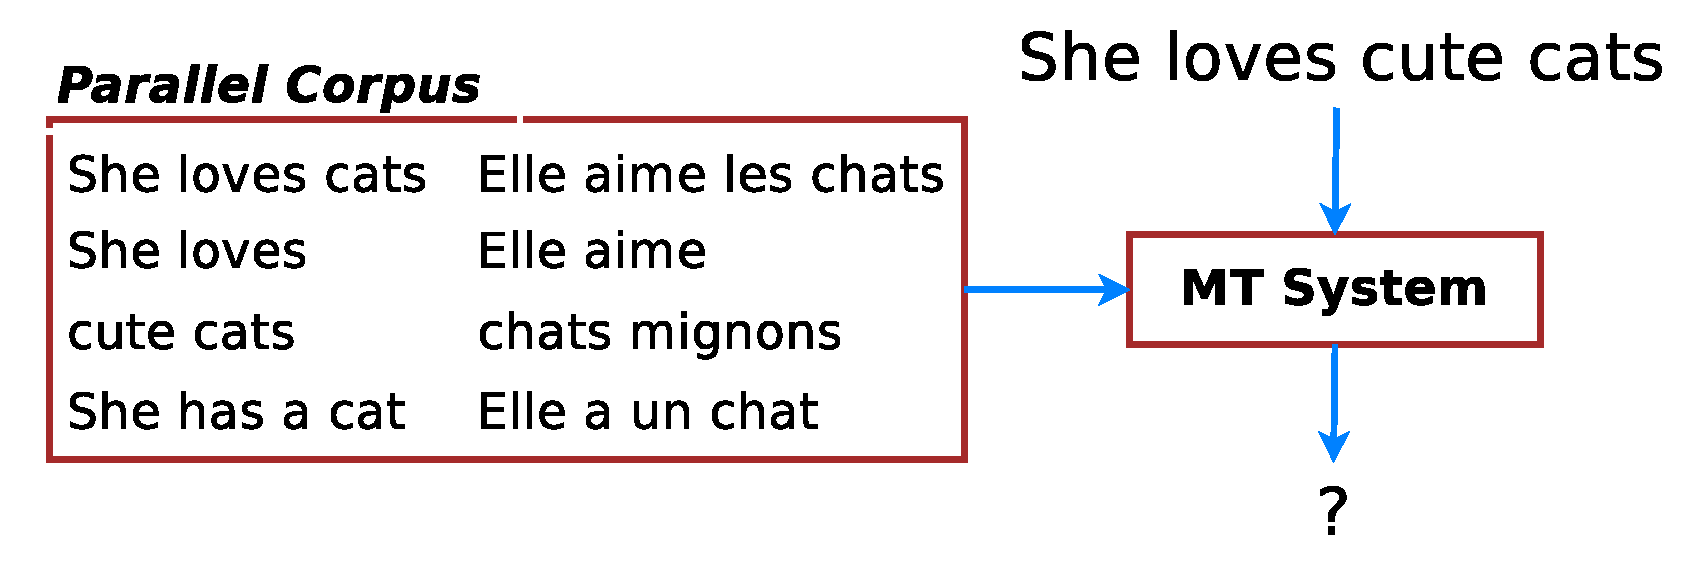
\includegraphics[width=0.6\textwidth, clip=true, trim= 0 0 0 0]{img/mt} % , angle=-90
\caption[A general setup of machine translation]{{\bf Machine translation} (MT) -- a general setup of MT. Systems
build translation models from parallel corpora to translate new unseen
sentences, e.g., \word{She loves cute cats}.}
\label{f:mt}
\end{figure}

Modern
statistical MT started out with a seminal work by IBM scientists
\cite{Brown:1993:MSM}. The proposed technique requires minimal linguistic
content and only needs a {\it parallel corpus}, i.e., a set of pairs of sentences that are translations of one
another, to train machine learning algorithms to tackle the translation problem.
Such a language-independent setup is illustrated in Figure~\ref{f:mt} and remains
to be the general approach for nowadays MT systems.
For over twenty years since the IBM seminal paper, approaches in MT
such as
\cite{Koehn:2003:SMT,och03,Liang:2006:EDA,koehn2007moses,chiang07hiero,dyer10cdec,cer10phrasal},
%inter alia, 
are, by and large, similar according to the following two-stage
process (see Figure~\ref{f:phrase_mt}). First, source sentences are broken into
chunks which can be translated in isolation by looking up a ``dictionary'', or
more formally a {\it translation model}. Translated target words and phrases
are then put together to form coherent and natural-sounding sentences by consulting a
{\it language model} (LM) on which sequences of words, i.e., {\it \ngram{}s}, are
likely to go with one another.

\begin{figure}[tbh!]
\centering
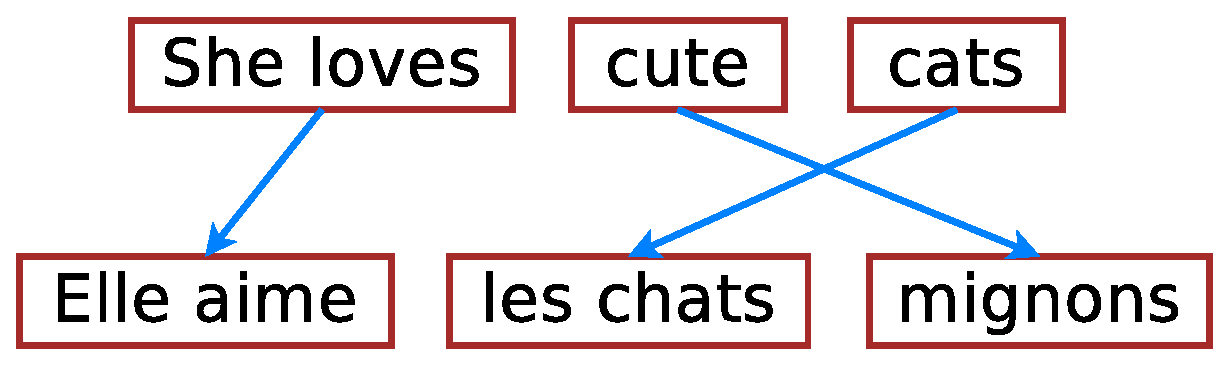
\includegraphics[width=0.45\textwidth, clip=true, trim= 0 0 0 0]{img/phrasemt} % , angle=-90
\caption[Phrase-based machine translation]{{\bf Phrase-based machine translation} (MT) -- example of how phrase-based
MT systems translate a source sentence \word{She loves cute cats} into a target sentence
\word{Elle aime les chats mignons}: sentences are split into chunks and phrases
are translated.
} 
\label{f:phrase_mt}
\end{figure}

The aforementioned approach, while has been successfully deployed in many commercial systems,
does not work very well and suffers from the following two major drawbacks.
First, translation decisions are {\it locally determined} as we translate
phrase-by-phrase and long-distance dependencies are often ignored. Second, it is
slightly ``strange'' that language models (LMs), despite being a key component in the MT
pipeline, utilize context information that is both short, consisting of only
a handful of previous words, and target-only, never looking at the source
words. These shortcomings in LMs gives rise to a new wave of {\it hybrid} systems which
aim to empower phrase-based MT with neural network components, most notably
neural language models (NLMs). 

NLMs were first proposed by \newcite{Bengio2003}
as a way to combat the ``curse'' of dimensionality suffered by traditional LMs.
In traditional LMs, one has to explicitly store and handle 
all possible \ngram{}s occurred in a training corpus, the number of which
quickly becomes enormous. As a result, existing MT systems often limit
themselves to use only short, e.g., $5$-gram, LMs \cite{kenlm}, which capture little context
and cannot generalize well to unseen \ngram{}s. NLMs address these concerns by
using distributed representations of words and not having to explicitly store
all enumerations of words. As a result, many MT systems, \cite{schwenk07,vaswani13decode,luong15nlm}, inter
alia, start adopting NLMs alongside with traditional LMs.
To make NLMs even more powerful, recent work \cite{Schwenk12continuous,devlin14}
propose to condition on source words beside the target context to lower
uncertainty in predicting next words (see Figure~\ref{f:nnjm}).\footnote{In
\cite{devlin14}, the authors have constructed a model that conditions on 3
target words and 11 source words, effectively building a $15$-gram LM.}
\begin{figure}[tbh!]
\centering
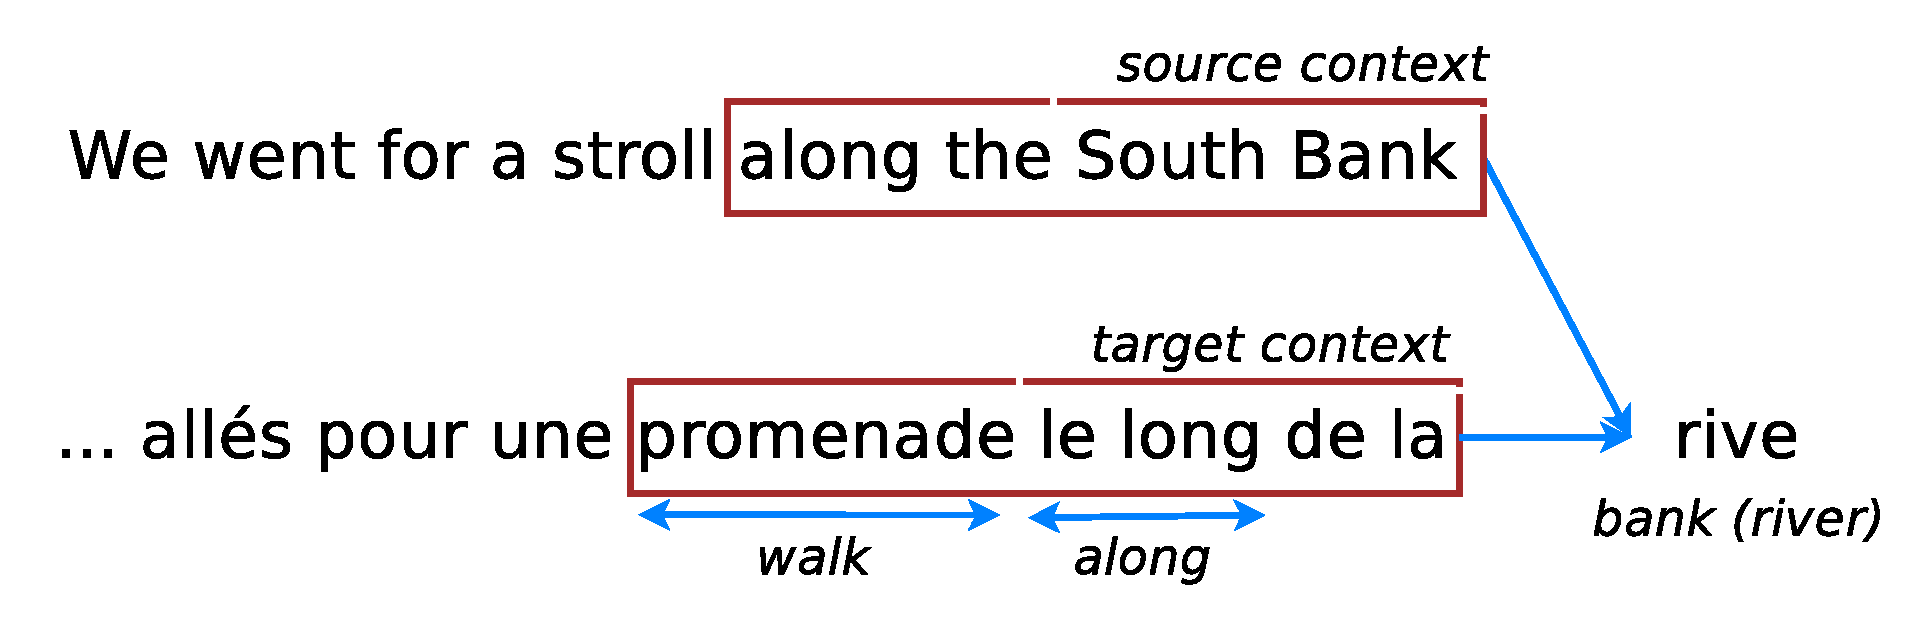
\includegraphics[width=0.7\textwidth, clip=true, trim= 0 0 0 0]{img/nnjm} % , angle=-90
\caption[Source-conditioned neural language model]{{\bf Source-conditioned neural language model} (NLM) -- example of a source-conditioned
NLM proposed by \newcite{devlin14}. To evaluate a how likely a next word
\word{rive} is, the model not only relies on previous target words (context)
\word{promenade le long de la} as in
traditional NLMs \cite{Bengio2003}, but also utilizes source context \word{along the
South Bank} to lower uncertainty in its prediction.
} 
\label{f:nnjm}
\end{figure}

These hybrid MT systems with NLM components, while having addressed shortcomings
of traditional phrase-based MT,
still translate locally and fail to capture long-range dependencies. For example, in Figure~\ref{f:nnjm}, the
source-conditioned NLM does not see the word \word{stroll}, or any other words
outside of its fixed context windows, which can be useful in deciding that the
next word should be \word{bank} as in \word{river bank} rather \word{financial
bank}. More problematically, the entire MT pipeline is already complex with
different components needed to be tuned separatedly, e.g., translation models,
language models, reordering models, etc.; now, it becomes even worse as
different neural components are incorporated. Neural Machine Translation to the
rescue!


Neural Machine Translation (NMT) is a new approach to translating text from one
language into another that captures long-range dependencies in sentences and
generalizes better to unseen texts. The core of NMT is a single deep neural
network with hundreds of millions of neurons that learn to directly map source
sentences to target sentences \cite{kal13,sutskever14,cho14}. 
%Despite being relatively new 
%\cite{kal13,sutskever14,cho14}, NMT has already shown promising results,
%achieving state-of-the-art performances for
%several language pairs such as
%English-French \cite{luong15}, English-German
%\cite{jean15,luong15attn,sennrich16mono}, and
%English-Czech \cite{jean15wmt,luong16}. 
This is often referred as the sequence-to-sequence or encoder-decoder
approach.\footnote{\newcite{forcada97} wrote the very first paper on sequence-to-sequence models for translation!}
NMT is appealing since it is conceptually
simple and can be trained
end-to-end. NMT translates as follows: an {\it encoder} reads through the given source
words one by one until the
end, and then, a {\it decoder} starts emitting one target
word at a time until a special end-of-sentence symbol is produced. We illustrate
this process in Figure~\ref{f:nmt}. 
% for the model described in \cite{sutskever14}.

\begin{figure}[tbh!]
\centering
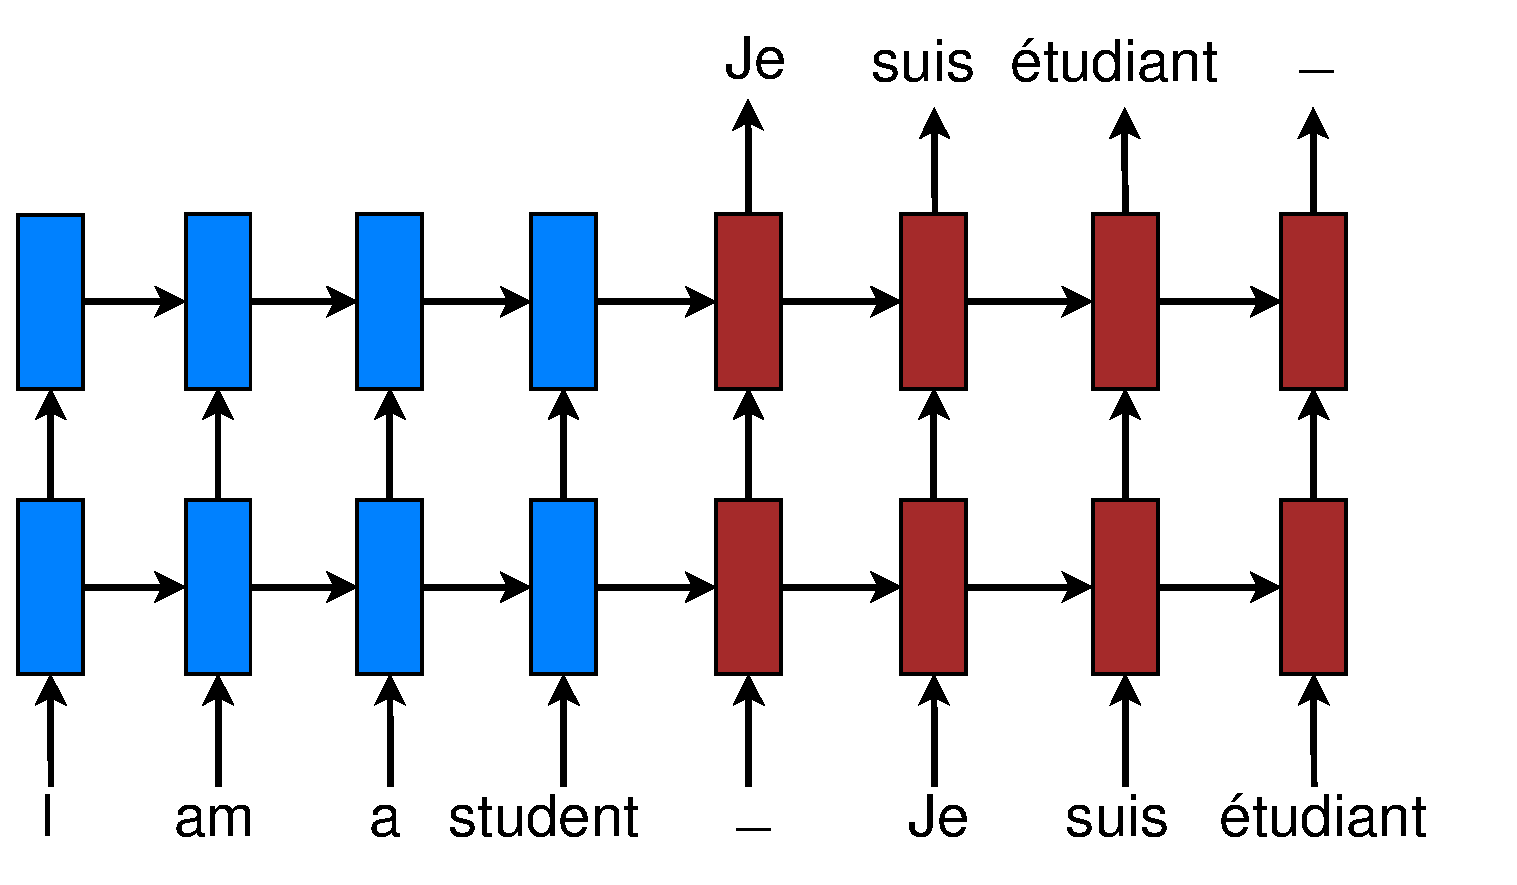
\includegraphics[width=0.6\textwidth, clip=true, trim= 0 0 0 0]{img/nmt_basic} % , angle=-90
\caption[Neural machine translation]{{\bf Neural machine translation} -- example of a deep recurrent
architecture proposed by \newcite{sutskever14} for
translating a source sentence \word{I am a student} into a target sentence
\word{Je suis \'{e}tudiant}. Here, \word{\texttt{\_}} marks the end of a sentence.
} 
\label{f:nmt}
\end{figure}

Such simplicity leads to several advantages. 
NMT requires minimal domain knowledge: it only assumes access to
sequences of source and target words as training data and learns to directly
map one into another. NMT beam-search decoders that
generate words from left to right can be easily implemented, unlike the highly
intricate decoders in standard MT \cite{Koehn:2003:SMT}. Lastly, the use of
recurrent neural networks (RNNs) allow NMT to generalize well to very long word
sequences while not having to 
explicitly store any gigantic
phrase tables or language models as in the case of standard MT.

Despite all these advantages and potentials, the early NMT architecture
\cite{sutskever14,cho14} still has many drawbacks. In this thesis, I will
highlight three problems pertaining to the existing NMT model, namely the
{\it vocabulary size}, the {\it sentence length}, and the {\it
language complexity} issues. Each chapter is devoted to solving each of these
problems in which I will describe how I have pushed the limits of NMT, making it
applicable to a wide variety of languages with state-of-the-art performance such as
English-French \cite{luong15}, English-German \cite{luong15attn,luong15iwslt}, and
English-Czech \cite{luong16}. Towards the {\it future} of
NMT, I answer two questions: (1) whether we can improve translation by jointly
learning from a wide variety of sequence-to-sequence tasks such as parsing,
image caption generation, and auto-encoders or skip-thought vectors
\cite{luong16iclr}; and (2)
whether we can compress NMT for mobile devices \cite{see16}.
In brief, this thesis is organized as follows. I start off by providing background knowledge on RNN and NMT
in Chapter~\ref{c:background}. 
The aforementioned three problems and approaches for NMT future are detailed in
Chapters~\ref{c:copy},~\ref{c:attention},~\ref{c:hybrid}, and~\ref{c:future}
respectively, which we will go through one by one next.
%My contributions are detailed in:
%Chapter~\ref{c:copy} on the rare word problem, Chapter~\ref{c:attention} on the
%sentence length problem, Chapter~\ref{c:hybrid} on the language complexity
%problem, and Chapter~\ref{c:future} on the future of NMT.
Chapter~\ref{c:conclude} wraps up and discusses remaining challenges in NMT research.

\subsubsection*{Copy Mechanisms} 
%\paragraph{Copy Mechanisms} 
A significant weakness in conventional NMT 
systems is their inability to correctly translate very rare words:  
end-to-end NMTs tend to have relatively small vocabularies with a single
\unk{} symbol that represents every possible out-of-vocabulary (OOV) word. In
Chapter~\ref{c:copy}, we propose simple and effective techniques to address this
{\it vocabulary size} problem through teaching NMT to ``copy'' words from source to
target. Specifically, we train an NMT system on data that is augmented by the output of a word 
alignment algorithm, allowing the NMT system to emit, for each OOV word
in the target sentence, the position of its corresponding word in the source sentence.
This information is later utilized in a
post-processing step that translates every OOV word using a dictionary.  Our
experiments on the WMT'14 English to French translation task show that this 
method provides a substantial improvement of up to 2.8 BLEU points over an
equivalent NMT system that does not use this technique. 
With 37.5 BLEU points, our NMT system is the first to surpass 
the best result achieved on a WMT'14 contest task.

\subsubsection{Attention Mechanisms} 
%\paragraph{Attention Mechanisms} 
While NMT can translate well for short- and medium-length sentences, it 
has a hard time dealing with long sentences.
An attentional mechanism was proposed by \newcite{bog15} to address that {\it
sentence length} problem by
selectively focusing on parts of the source sentence during translation. However,
there has been little work exploring useful architectures for attention-based
NMT. Chapter~\ref{c:attention} examines two simple and effective classes of attentional
mechanism: a {\it global} approach which always attends to all source words and
a {\it local} one that only looks at a subset of source words at a time. 
We demonstrate the effectiveness of both approaches on the WMT translation
tasks between English and German in both directions. With local
attention, we achieve a significant gain of 5.0 BLEU points over
non-attentional systems that 
already incorporate known techniques such as dropout. Our ensemble 
model using different attention architectures yields a new
state-of-the-art result in the WMT'15 English to German
translation task with 25.9 BLEU points, an improvement of 1.0 BLEU points over the existing
best system backed by NMT and an $n$-gram reranker.

\subsubsection{Hybrid Models} 
%\paragraph{Hybrid Models} 
Nearly all previous NMT work has used quite restricted
vocabularies, perhaps with a subsequent method to patch in unknown words such as
the copy mechanisms mentioned earlier. While effective, the copy mechanims cannot deal with all the
complexity of human languages such as rich morphology, neologisms, and informal
spellings.
Chapter~\ref{c:hybrid} presents a novel word-character solution to that {\it
language complexity} problem towards achieving
open vocabulary NMT.
We build hybrid systems that translate mostly at the {\it word}
level and consult the {\it character} components for rare words. 
Our character-level recurrent neural networks compute source
word representations and recover unknown target words when needed.
The twofold advantage of such a hybrid approach is that it is much faster and easier to
train than character-based ones; at the same time, it never produces unknown words as in the case of word-based models. 
On the WMT'15 English to Czech translation task, 
this hybrid approach offers an addition boost of +$2.1{-}11.4$ BLEU points over models 
that already handle unknown words. 
Our best system achieves a new state-of-the-art result with
$20.7$ BLEU score.
We demonstrate that our character models can successfully learn to not only generate well-formed words for Czech, a
highly-inflected language with a very complex vocabulary, but also build correct
representations for English source words.

\subsubsection{NMT Future} 
%\paragraph{NMT Future} 
Chapter~\ref{c:future} answers the two aforementioned questions
for the future of NMT: whether we can utilize other tasks to improve
translation and whether we can compress NMT models.
%, I answer two questions in Chapter~\ref{c:future}: (1) whether we can improve translation by jointly
%learning from a wide variety of sequence-to-sequence tasks such as parsing,
%image caption generation, and auto-encoders or skip-thought vectors; and (2)
%whether we can compress NMT for mobile devices.

For the first question, 
we examine three multi-task learning (MTL) settings for sequence to sequence
models:
(a) the {\it one-to-many} setting -- where the encoder is shared
between several tasks such as machine translation and
syntactic parsing, (b) the {\it many-to-one} setting -- useful when only the
decoder can be shared, as in the case of 
translation and image caption generation, and (c) the {\it
  many-to-many} setting -- where multiple encoders and decoders are
shared, which is the case with unsupervised objectives
and translation.  Our results show that training on a small amount of parsing and
image caption data can improve the translation quality between English and
German by up to $1.5$ BLEU
points over strong single-task baselines on the WMT benchmarks. Rather
surprisingly,
we have established a new {\it
state-of-the-art} result in constituent parsing with 93.0 F$_1$ by utilizing
translation data. Lastly, we reveal interesting properties of the two unsupervised learning
objectives, autoencoder and skip-thought, in the MTL context: autoencoder helps less in terms of
perplexities but more on BLEU scores compared to skip-thought.

%Neural Machine Translation (NMT), like many other deep learning domains, typically suffers from over-parameterization, resulting in large storage sizes.
For the second question, we examine three simple magnitude-based pruning schemes to compress NMT models, namely {\it class-blind}, {\it class-uniform}, and {\it class-distribution}, which differ in terms of how pruning thresholds are computed for the different classes of weights in the NMT architecture.
We demonstrate the efficacy of weight pruning as a compression technique for a state-of-the-art NMT system. 
We show that an NMT model with over 200 million parameters can be pruned by 40\% with very little performance loss as measured on the WMT'14 English-German translation task. 
This sheds light on the distribution of redundancy in the NMT architecture.
Our main result is that with {\it retraining}, we can recover and even surpass the original performance with an 80\%-pruned model. 


%We start off by providing background knowledge on RNN and NMT
%in Chapter~\ref{c:background}. The following chapters detail my contributions.
%Chapter~\ref{c:copy} discusses how the rare word
%problem in NMT is addressed with a mechanism to ``copy'' words from source to
%target; hence, extending the vocabulary
%coverage. Chapter~\ref{c:attention} describes
%how the attention mechanism, a way to select
%local contexts in the source sentence as we transate, can be effectively used in
%NMT to better handle long sentences. Chapter~\ref{c:hybrid} 
%proposes a novel way of dealing with language complexity (rich morphology,
%neologisms, and informal spellings) by building a hybrid word and character
%level model which can gain from the flexibility of a character-level model while
%maintaining the speed and quality of the word-level model. Towards the future of
%NMT, I answer two questions in Chapter~\ref{c:future}: (1) whether we can improve translation by jointly
%learning from a wide variety of sequence-to-sequence tasks such as parsing,
%image caption generation, and auto-encoders or skip-thought vectors; and (2)
%whether we can compress NMT for mobile devices.
%Chapter~\ref{c:conclude} wraps up and discusses remaining challenges in NMT
%research.


%Due to computational constraint, NMT has to limit its vocabulary to a fixed set
%of top frequent words, e.g., the top 50K words. As a result, all other words
%are represented by a universal symbol \unk{}.
%
%I discuss in Chapter~\ref{c:copy} discusses how the rare word
%problem in NMT is addressed with a mechanism to ``copy'' words from source to
%target; hence, extending the vocabulary
%coverage.

